\documentclass[letterpaper, 12pt]{report}
\usepackage[utf8]{inputenc}
\usepackage[margin=1in,letterpaper]{geometry}
\usepackage[stretch=10]{microtype}
\renewcommand{\baselinestretch}{1.5}
\usepackage{fancyhdr}
\setlength{\headheight}{15pt}
\pagestyle{fancy}
\usepackage{amsmath}
\usepackage{siunitx}
\usepackage{url}
\urlstyle{same}
\usepackage{graphicx}
\usepackage{caption}
\usepackage{subcaption}
\usepackage{cite}
\usepackage{listings}
\usepackage[table,xcdraw]{xcolor}
\usepackage{listings}
\usepackage{color}
\usepackage[final]{pdfpages}
\definecolor{navy}{rgb}{245,156,74}
\definecolor{codegreen}{rgb}{0,0.6,0}
\definecolor{codegray}{rgb}{0.5,0.5,0.5}
\definecolor{codepurple}{rgb}{0.58,0,0.82}
\definecolor{backcolour}{rgb}{0.95,0.95,0.92}
\lstdefinestyle{mystyle}{
    backgroundcolor=\color{backcolour},   
    commentstyle=\color{codegreen},
    keywordstyle=\color{magenta},
    numberstyle=\tiny\color{codegray},
    stringstyle=\color{codepurple},
    basicstyle=\footnotesize,
    breakatwhitespace=false,         
    breaklines=true,                 
    captionpos=b,                    
    keepspaces=true,                 
    numbers=left,                    
    numbersep=5pt,                  
    showspaces=false,                
    showstringspaces=false,
    showtabs=false,                  
    tabsize=2
}
\lstset{style=mystyle}
\usepackage[outdir=./]{epstopdf}
\usepackage{tcolorbox}
\tcbuselibrary{skins,breakable}
\usepackage{nomencl}
\makenomenclature
\usepackage{hyperref}
\hypersetup{
    colorlinks=true,
    linkcolor=-navy,
    filecolor=blue,      
    urlcolor=blue,
    runcolor=red,
    citecolor=green,
}

\begin{document}
\begin{titlepage}
    \begin{center}
        \vspace*{1cm}
            
        \large
        \textbf{REACTION CONTROL SYSTEM FOR HIGH ALTITUDE BALLOONS}
            
        \vspace{0.5cm}
        \normalsize
        Characterizing the Cold Gas Thruster for Reaction Control
            
        \vspace{1.5cm}
            
        Max Huggins\\
        

            
        \vfill
            
        A thesis presented in partial fullfillment for\\
        Honors in the Bachelor's of Science Degree
            
        \vspace{0.8cm}
            
        \includegraphics[width=0.4\textwidth]{Figures/UCA}
            
        Faculty Mentor: William Slaton\\
        Reader: ??\\
        Department of Physics and Astronomy\\
        University of Central Arkansas\\
        \today
            
    \end{center}
\end{titlepage}
\thispagestyle{plain}
\begin{center}
    \large
    \textbf{Reaction Control System for High Altitude Balloons}
        
    \vspace{0.4cm}
    \normalsize
    Characterizing the Cold Gas Thruster for Reaction Control
        
    \vspace{0.4cm}
    \textbf{Max Huggins}
       
    \vspace{0.9cm}
    \textbf{Abstract}
\end{center}
Several methods exist which allow scientists to collect various types of data from Earth's atmosphere. High altitude balloons are one of these methods, which provide scientists a cost effective, simple system for data collection. At the cost of simplicity, however they lack control. Sporadic winds in the atmosphere affect data collection for sensors on board these balloon's payloads. A reaction control system would allow stabilization through regions of the atmosphere to allow better data collection. Here, the development of a reaction control system utilizing cold gas thrusters has been outlined. From the decision of fuel to the methods of characterization. An analysis has been done to characterize the behaviour of the thrusters, but due to an incomplete data set the characterization was unable to be completed. A high-level outline on future work has been laid out along with the experimental and analytical scripts.
\clearpage
\section*{COVID-19}
This was a two semester project, performed in last year of a Bachelor's of Science Degree. The first semester was spent working to develop the background knowledge and the experiment. The second was spent actually setting up the experimental apparatus and data acquisition system; as well as collecting data. However, the University of Central Arkansas began online instruction March 13, 2020 and access to the research labs was limited due to COVID-19. Because of this, some necessary data collection was not completed and progress on the project was halted. The analysis and results that could be completed are discussed here. \\
In hopes of future work being completed, an outline will be presented for later work to be done.

\tableofcontents
\printnomenclature[0.5in]

\chapter{Introduction}\label{chap:Introduction}
\section{Background}
High altitude balloons (HABs) are large balloons to which one or several payloads are attached that can reach high altitudes. These payloads are insulated packages typically holding scientific equipment for data collection. Here, high altitude balloon payloads will be referred to as HABPs. Some examples of sensors that may be on board the HABPs are: temperature, altitude, pressure, wind, radiation, and so on. These can provide information for meteorologists and researchers about conditions in high levels of the atmosphere with prolonged data collection. This is unlike other methods of atmospheric data collection like rockets which can also reach these altitudes but do it over a much shorter time-span. HABs can also provide safer, more cost effective options for data collection. However, there are some downfalls of using balloons as a means of data collection. They can be subject to high winds and any on board sensors will be affected by this. For example, during the 2017 total solar eclipse any payloads sent up to observe this would have been subject to winds throughout their flight. This means that camera footage observing the sun's corona would never be stable and set on the subject it is observing. The cameras would be passive observers controlled by the wind rather than the scientist. Another example is Geiger counters observing radiation in the atmosphere. These may have inconsistent data depending on what part of the payload is in its path from the sun. Wind speed sensors will also be subject to the forces of the winds. Keeping up with the inconsistent direction of the payload is a difficult task and the sensor is provided wind speed that is not in any particular direction. This is not ideal to determine the direction of the winds and would require much post-processing to match up the direction the payload was facing at a given wind speed data point. These are only three specific examples, but winds will affect many other data collection systems. The goal of this project is to develop a system that stabilizes the payload against wind speeds.
\section{Outline}
The ultimate objective here is to fly a reaction control system on board a HABP. Getting to this point requires several steps. A high-level overview is listed:
\begin{enumerate}
\item Determining viability of different RCSs
\item Choosing a RCS
\item Characterizing the chosen RCS
\item Implementing the RCS
\item Ultimate objective
\end{enumerate}
\subsection{Options}
The relevant options that were considered for the RCS can be divided into two categories. The first is of the gyroscopic type. These can offer both passive an active stabalization. Reaction wheels (RWs) are commonly used in satellites and telescopes in order to change the attitude of a craft with extreme accuracy. There are also control moment gyroscopes (CMGs) which are essentially reaction wheels mounted on a gimbal controlled by a motor. These produce much higher torques than RWs and more typically provide active stabilization. Both CMGs and RWs rely on electricity as their energy source; while crafts like the International Space Station along with others can utilize solar panels for the longevity of missions, HABs cannot. They would rely on a battery to store all of the energy used to move the craft. Another drawback to these gyroscopic systems is their slow reaction time. These are typically not used for stabilizing a craft throughout a flight. Rather they provide reactions to torques from solar radiation pressure, gravity gradient, magnetic fields, micrometeorite impact, and internal effects like gas leakage and moving parts \cite{electricvthruster}. In the case of these scenarious it is not a matter of time and unpredictability. Additionally, they rely on motors spinning up to change the direction of the craft which takes considerable time. The other type of option consdiered here is the thruster type. This takes the form of both combustion and cold gas thrusters. These cannot offer the same amount of accuracy as the former, but can provide extremely fast changes in momentum. They are more commonly used for stabalizing crafts utilizing rockets and rely on compressed air energy storage (CAES) or chemical energy storage rather than electricity.\\
Of the two, the thruster types have more desireable properties. Primarily in their ability to provide faster changes in the attitude of the craft. Now, the consideration to be made is between the combustion or cold gas thruster. Obviously, sticking combustible fuel on board a HAB is not considered safe so the CGT is more desireable. Also, the design of a CGT system (CGTS) has a lower level of complexity. The choice of system for this project is the CGT.
\subsection{Fuel Options}
An in-depth analysis was not necessarily done regarding the choice of the CGT for stabalization in the previous section. So it is important to determine the viability of several types of common fuels. To determine the viability of a CGT, a variable called the specific impulse ($I_{sp}$) must be defined. Equation \ref{eq:SpecificImpulse} provides the definition of the specific impulse.
\begin{equation}\label{eq:SpecificImpulse}
I_{sp}=\frac{F}{dm_p/dt}
\end{equation}%
\nomenclature{$I_{sp}$}{The specific impulse}%
\nomenclature{$F$}{Force or thrust}%
\nomenclature{$m_p$}{Mass of propellant}%
\nomenclature{$t$}{Time}\\
Where $F$ is the force and $dm_p/dt$ is the change in mass of propellant with respect to time. This value provides a \textit{standard} so to speak for characterizing fuels as it describes the force production per some amount of mass of a fuel. Different fuels have different $I_{sp}s$ and generally speaking the higher the value the better the fuel. \footnote{It is worth noting the units for $I_{sp}$ are $Ns/kg$, but most sources will record the value in units of $s$. While this is not necessarily true to the definition, all that they are doing is multiplying $m_p$ by the acceleration due to gravity and this makes no difference for the purpose the $I_{sp}$ is serving here.} Additionally, given an impulse, the amount of fuel required to counteract an impulse can be determined. This describes stabalization well. Looking at some sample data from \cite{titan1hab}, the amount of fuel required to stabilize a flight can be estimated. The raw flight data was not given in form of a .txt or .csv, but plots of the raw data are shown. From this, a digitizer tool was used to extract numbers from the gyroscopic plots. Specifically, the angular velocity about the axial direction ($\omega_z$). Multiplying this by the radius of rotation ($r$) and then taking the derivative with respect to time gives the accerlation ($a_w$) due to the forces ($F_w$) of the wind. Multiplying this by the mass of the payload ($m_{pd}$) then determines the force in the relevant direction due to the wind. Using the theoretical values for the specific impulse of different gases, the mass of fuel needed for a flight could be determined. In other words,
\begin{equation}\label{eq:alpha}
a_w = \frac{d(\omega_z r)}{dt}
\end{equation}%
\nomenclature{$a_w$}{Acceleration caused by wind}%
\nomenclature{$r$}{Radius}%
\nomenclature{$\omega_z$}{Angular velocity about z axis}
\begin{equation}\label{eq:windforce}
F_w = m_{pd}a_w
\end{equation}%
\nomenclature{$F_w$}{Force caused by wind}%
\nomenclature{$m_{pd}$}{Mass of the payload}
The integration of all these values would provide the total impulse caused by the wind ($I_w$).
\begin{equation}\label{eq:windimpulse}
I_w=\int |F_w| dt
\end{equation}%
\nomenclature{$I_w$}{Impulse caused by wind}
\begin{equation}\label{eq:propmass}
m_p=\frac{I_w}{I_{sp}}
\end{equation}
In reality equations \ref{eq:alpha}, \ref{eq:windforce}, and \ref{eq:windimpulse} are performed for each data point throughout the data set. The derivative is the difference in two points next to each other and the integral is a trapezoidal sum throughout the flight. Also, since the force would take both positive and negative values, the absolute value of each force term was taken.
\subsubsection{Fuels}
The most commonly used gas in a CGT is by far nitrogen; the reason for this is reasonable  propellant storage density, performance and lack of contamination concerns \cite{thrusteroptions}. Some other options are $CO_2,\ H_2,\ and\ He$; $H_2$ having the highest specific impulse. Obviously, the specific impulse is not the only important variable when considered what makes the best fuel for a system. Factors such as safety, availability, cost, energy storage density, and so on all contribute to the choice of gas. The theoretical specific impulse values of the gases listed above are shown in table \ref{tab:GasIsps}. Along with the specific impulse, the mass required for each gas to stabilize the payload for the total trip is recorded. 
\begin{table}[!h]
\centering
\begin{tabular}{
>{\columncolor[HTML]{C0C0C0}}c 
>{\columncolor[HTML]{EFEFEF}}c 
>{\columncolor[HTML]{EFEFEF}}c 
>{\columncolor[HTML]{EFEFEF}}c }
$Gas$  & \cellcolor[HTML]{C0C0C0}$I_{sp}\ (s)$ & \cellcolor[HTML]{C0C0C0}$Mass\ (g)$ & \cellcolor[HTML]{C0C0C0}$Mass\ Ozone\ (g)$ \\
$H_2$  & 296                                   & 172                                 & 5                                          \\
$He$   & 179                                   & 284                                 & 8                                          \\
$N_2$  & 80                                    & 636                                 & 18                                         \\
$CO_2$ & 67                                    & 760                                 & 21                                        
\end{tabular}
\label{tab:GasIsps}
\end{table}
In the third column, the mass of fuel needed for the time the payload spends in the ozone layer is also recorded. It is not always necessary to stabilize the payload throughout the entirety of the flight. In fact, the target may be a specific altitude region so in this case stabilization in other regions is irrelevant. To put these numbers into perspective, the $CO_2$ cannisters that mountain bikers use to refill their tires are typically 16g cartridges. The $CO_2$ and the cartridge together weigh approximately 60g. The maximum mass allowed by the FDA for the type of HABP dealt with here is 2721.554g; meaning one of these 16g cartridges is only approximately 2\% the total mass of the payload. A 25g cartride is still only approximately 3.8\% the total mass and well within the volume constraints as well. So, at a high-level view, the CGTS is a seemingly viable option.\\
Since several trials will be recorded availability of the gas is largely important to this project. Out of these gases the availability of $CO_2$ is by far the highest. Even with the lowest $I_{sp}$, it is still an attractive option. Additionally, the actual implementation of the CGT is a distance away from this point in the project. As each gas should behave similarly in the system, it would not be a difficult task to switch the type of gas at any given point during the project. If further analysis finds the specific impulse to be of more importance then $N_2$ would be the most likely option for the aforementioned reasons. 
\section{Characterizing}
The characterization of the RCS is referring to fitting the actual results of the system to the pre-exisisting theory's results. This is reffering to the theory discussed in chapter \ref{chap:Theory}. From a high-level, it is likely the assumptions made to generate the mathematical equations do not fit the actual behaviour of the system. In fact, the book, reference \cite{langton}, from which the actual nozzle theory is taken states the theory produces an error of approximately 12\% for actual rocket engines. [*****CHECKTHISS] The goal in characterizing the system is to create a proportionality between the predicted and actual results in order to specify the predicted results for the system developed here. To accomplish this, an on-ground testing rig is built consisting of the same parts to be integrated into the actual payload. The on-ground rig measures variables of interest in the system that will allow the comparison between the predicted and actual results. This will be discussed in more detail in chapter \ref{Methods}, section \ref{Characterizing}. In the high-level outline provided, this is the section where progress was halted due to the COVID-19 crisis. From this point further in the project is considered an outline for future work.
\section{Integration}
After characterization of the system, the actual integration into a HABP must be made. This is a straightforward task and involves adding another thruster and solenoid to the on-ground testing rig and removing some sensors that are no longer necessary. Then fitting the plumbing into the HABP. Additionally, the scripting for stabilization must be developed further and specified for the characteristics determined. A CAD rendering of the plumbing system is shown in figure \ref{fig:CAD}.
%\begin{figure}[h!]
%\centering
%\includegraphics[scale=.5]{Figures/CAD}
%\caption{CAD rendering of the plumbing system to be used in the actual payload}
%\label{fig:CAD}
%\end{figure}
This integration would include simulating windy conditions and determining impulse data from accelerometer sensors to see how the system would work for actual flights. As well as determining the type of feedback system to be used for the RCS script. Examples of these are all negative feedback systems using some type of sensor such as a magnetometer, photoresistor, accelerometer, etc to provide the controller a reference for the pointing direction. This is the point where the amount of fuel needed for a flight objective could be well defined and the necessary changes could be implemented.
\section{Flight}
After confidence in the system has been established from the on-ground testing and simulations, the goal and best test is a flight of the RCS. Here, it is important that the sytem is integrated with a data acquisition system and acts as an aid in the data acquisition. The flight objective has not been well-defined yet. Some vague examples are listed:
\begin{itemize}
\item "Look" at a ground target for a duration of the flight
\item Take footage of only the sun for a duration of flight
\item Record radioactivity with the sensor unobstructed towards the sun through the ozone layer
\end{itemize}
The system should be robust enough such that completion of these tasks is not a matter of altering the CGTS in any way, but rather altering the scripting and feedback system. 

\chapter{Theory}\label{chap:Theory}
The objective of this section is to derive the relationships used for the analysis of the data collection. First, the general thermodynamic relationships will be established, then they will be applied to converging-diverging nozzle. At this point, the relevant relationships for the data will be established and the experimental design can be discussed in detail.
\section{General Thermodynamic Relationships}
The theory used here is mostly taken from pre-existing nozzle theory. The source for this project is reference \cite{langton}. Much of the derivation for the equations to be used are based on the following assumptions and rely on Classical Thermodynamics:
\begin{enumerate}
\item The propellant is homogeneous throughout the nozzle.
\item The propellant behaves like a perfect gas.
\item There is no friction between the propellant and the nozzle walls
\item The system is adiabatic
\item The propellant flow is one-dimensional
\item The propellant flow is stagnate in the nozzle chamber
\item The propellant velocity is uniform accros any cross-section normal to the nozzle axis
\end{enumerate}
Reference \cite{langton} refers to three other assumptions, but they either do not apply or are redundant for the CGTS. Additionally, all of the variables are clearly defined in the nomenclature section but will not be defined along the discussion here.\\
Starting with the first law of thermodynamics (FLT),
\begin{equation}\label{eq:FLT}
dQ=dU+PdV
\end{equation}%
\nomenclature{$Q$}{Heat put into a system}%
\nomenclature{$U$}{Internal energy}%
\nomenclature{$V$}{Volume}%
\nomenclature{$P$}{Pressure}%
\nomenclature{$X_x$}{Represents some variable, X, at some point x}%
\nomenclature{$X_i$}{Represents some variable, X, at some initial state}%
\nomenclature{$X_f$}{Represents some variable, X, at some final state}
\nomenclature{$X_s$}{Represents some variable, X, at stagnation}%
\nomenclature{$X_c$}{Represents some variable, X, in the nozzle chamber}%
\nomenclature{$X_t$}{Represents some variable, X, in the nozzle throat}%
\nomenclature{$X_e$}{Represents some variable, X, in exit plane of the nozzle}%
and according to the second law,
\begin{equation}\label{eq:SLT}
dQ=TdS
\end{equation}%
\nomenclature{$T$}{Temperature}%
\nomenclature{$S$}{Entropy}
defining the specific heats at constant volume and pressure respectively,
\begin{equation}\label{eq:SHV}
c_V=\left(\frac{\partial Q}{\partial T}\right)_V
\end{equation}
\begin{equation}\label{eq:SHP}
c_P=\left(\frac{\partial Q}{\partial T}\right)_P
\end{equation}
and using Joule's equation to define a perfect gas
\begin{equation}\label{eq:Joule}
\left(\frac{\partial U}{\partial V}\right)_T=0
\end{equation}
substitutting \ref{eq:FLT} into $\partial Q$ in \ref{eq:SHV}
\begin{equation}
c_V=\left(\frac{\partial U}{\partial T}\right)_V
\end{equation}
Also, substitutting \ref{eq:SLT} into $\partial Q$ in \ref{eq:SHV}
\begin{equation}
c_V=T\left(\frac{\partial S}{\partial T}\right)_V
\end{equation}
so
\begin{equation}\label{eq:cV}
c_V=\left(\frac{\partial U}{\partial T}\right)_V=T\left(\frac{\partial S}{\partial T}\right)_V
\end{equation}
similarly with $c_P$
\begin{equation}\label{cP}
c_P=\left(\frac{\partial U}{\partial T}\right)_P=P\left(\frac{\partial V}{\partial T}\right)_P
\end{equation}
this means \ref{eq:SLT} can be written as
\begin{equation}\label{eq:NewSLT}
dQ=c_VdT+PdV
\end{equation}
Considering a perfect gas, the equation of state is
\begin{equation}\label{eq:IGL}
PV=nRT
\end{equation}%
\nomenclature{$R$}{Universal gas constant}%
\nomenclature{$n$}{Number of moles}
substitutting $n=m/W$ provides%
\nomenclature{$W$}{Molecular weight of the gas}
\begin{equation}
PV=\frac{mRT}{W}
\end{equation}
so the equation for 1 unit of mass is
\begin{equation}\label{eq:IGL1}
PV=\frac{RT}{W}
\end{equation}
differentiating $PV$ gives
\begin{align}
d(PV)&=VdP+PdV\\
&=\frac{R}{W}dT
\end{align}
so
\begin{equation}\label{eq:NewSLTinIGL}
PdV=\frac{R}{W}dT-VdP
\end{equation}
Defining a new constant, $\gamma$
\begin{equation}\label{eq:Gamma}
\gamma=\frac{c_P}{c_V}
\end{equation}%
\nomenclature{$\gamma$}{Ratio of specific heats}
from this, \ref{eq:NewSLTinIGL}, \ref{eq:NewSLT}, and \ref{eq:SHP}
\begin{equation}\label{eq:GammaincV}
c_V=\frac{R}{W(\gamma-1)}
\end{equation}
similarly,
\begin{equation}\label{eq:GammaincP}
c_P=\frac{\gamma R}{W(\gamma-1)}
\end{equation}
It can also be determined for an adiabat, $dQ=0$, that
\begin{equation}\label{eq:adiabat}
P_iV_i^{\gamma}=P_fV_f^{\gamma}
\end{equation}
From the previous relations and the definition of enthalpy,
\begin{equation}\label{eq:Enthalpy}
H=U+pV
\end{equation}%
\nomenclature{$H$}{Enthalpy}
the enthalpy per unit mass can now be expressed as
\begin{equation}\label{eq:Enthalpypermass}
H=\frac{\gamma RT}{W(\gamma-1)}
\end{equation}
\section{The Nozzle}
Until this point, all of these relations are quite general. Figure \ref{fig:Nozzle} displays a typical converging diverging nozzle. It consists of three important regions. The furthest left is the chamber, it is here that we assume the variables to be stagnate. Stagnate meaning the velocity of the gas is zero. The next section going in the $+x$ direction is the nozzle throat. This is the smallest cross-sectional area of the system. Next is not a particularly important point, but represents the variables at any point, x, in the nozzle. Lastly is the exit plane of the nozzle. 
\begin{figure}[h!]
\centering
\includegraphics[scale=1]{Figures/Nozzle}
\caption{Simplified nozzle, with axis and some variables defined.}
\label{fig:Nozzle}
\end{figure}
To apply the previous definitions to a nozzle, the kinetic energy of 1 unit of mass will be considered along with the enthalpy. If the flow of the gas is considered, the enthalpy will increase by the amount equal to the kinetic energy of the gas per 1 unit of mass, given the gas exchanges no heat with the environment
\begin{align}
KE&=\frac{v^2}{2}\\
H_x&=\frac{\gamma RT_x}{W(\gamma-1)}\\
H_f&=H_x + KE
\end{align}%
\nomenclature{$KE$}{Kinetic energy}
A region where the gas is stagnant ($v=0$) can be considered, here the enthalpy is a constant. Substitutting \ref{eq:IGL1} and the specific volume ($V=1/\rho$) as well,
\begin{align}\label{eq:CasH}
H_s=C&=\frac{\gamma P_s}{W\rho_s(\gamma-1)}\\
&=\frac{\gamma}{(\gamma-1)}\frac{P_x}{W\rho_x}+\frac{v_x^2}{2}
\end{align}%
\nomenclature{$C$}{A constant relevant to the enthalpy at stagnation}
Now, considering an adiabatic system
\begin{equation}\label{eq:Adiabat}
\frac{V_s}{V_x}=\left(\frac{P_x}{P_s}\right)^{\frac{1}{\gamma}}
\end{equation}
From \ref{eq:CasH} and \ref{eq:Adiabat} it can be found that
\begin{equation}\label{eq:1.20}
\frac{P_x}{P_s}=\left(1-\frac{v^2}{2C}\right)^{\frac{\gamma}{\gamma-1}}
\end{equation}
\subsection{Mach Number}
An important parameter is the mach number, which is defined as the ratio of the gas velocity at some point to the velocity of sound in the gas. Here, this will be manipulated to determine the parameter in terms of temperature variables.
\begin{align}\label{eq:DefineMach}
M_x&=\frac{v_x}{v_{sound}}\\
&=\frac{v_x}{\sqrt{\gamma R T_x}}\\
\end{align}%
\nomenclature{$M$}{Mach number}
This can be substitutted into the previously defined relationships to find
\begin{equation}\label{eq:1.25}
\frac{T_s}{T_x}=1+M_x^2\frac{\gamma-1}{2}
\end{equation}
From \ref{eq:SHP} and the fact that the net heat change is equal to the change in kinetic energy per unit mass, the
\begin{align}
dQ&=c_PdT\\
&=c_P(T_x-T_{x+dx})\\
&=\frac{(v_{x+dx}^2-v_x^2)}{2J}
\end{align}
Where $J$ is defined as
\begin{equation}
J=\frac{W}{Q}
\end{equation}%
\nomenclature{$W$}{Work}
\nomenclature{$J$}{The mechanical equivalent of heat}
Substitutting \ref{eq:GammaincP}, using the stagnation conditions for the initial values, and solving for $v_x$,
\begin{equation}\label{eq:GasVelocity}
v_x=\sqrt{\frac{2\gamma RT_s}{(\gamma-1)W}\left(1-\left(\frac{P_x}{P_s}\right)^{\frac{\gamma-1}{\gamma}}\right)}
\end{equation}
Now, the velocity of the gas at any point x is in terms of variables in regions where flow is stagnated. The temperature can be found similarly,
\begin{equation}\label{eq:GasTemp}
T_x=T_s-\frac{v_x^2}{2Jc_P}
\end{equation}
substitutting \ref{eq:GasVelocity} and \ref{eq:GasTemp} into the mach number
\begin{equation}\label{eq:MachInTermsofT}
M^2=\frac{2}{(\gamma-1)}\left(\frac{T_s}{T_x}-1\right)
\end{equation}
Lastly,
\begin{equation}\label{eq:MRatio}
\frac{M_{x+dx}}{M_x}=\frac{v_{x+dx}}{v_x}\sqrt{\frac{T_x}{T_{x+dx}}}
\end{equation}
\subsection{Area Ratio}
The expansion ratio is the single most important parameter when designing an efficient nozzle. This is the ratio of the exit plane area to the throat plane area. To introduce the variable, the mass flow rate will be defined.
\begin{equation}\label{eq:MassFlow}
w=\frac{dm}{dt}
\end{equation}
In terms of the geometry of the nozzle, the velocity of the gas, and the density
\begin{equation}
w=A_xv_x\rho_x
\end{equation}%
\nomenclature{$\rho$}{Density}
The mass flow rate must be constant throughout any given time in the system. This is the equation of continuity for the flow. The ratio of any two points for a unit mass can now be analyzed,
\begin{equation}\label{eq:MassFlowwDensity}
\frac{A_{x+x}}{A_x}=\frac{V_{x+dx}v_x}{V_xv_{x+dx}}
\end{equation}
Using \ref{eq:Adiabat} for the general case, \ref{eq:MachInTermsofT}, and \ref{eq:MRatio}
\begin{equation}
\frac{A_{x+dx}}{A_x}=\frac{M_x}{M_{x+dx}}\left(\frac{T_x}{T_{x+dx}}\right)^\frac{1}{2}\left(\frac{1+\frac{(\gamma-1)}{2}M_{x+dx}^2}{1+\frac{(\gamma-1)}{2}M_x^2}\right)^{\frac{1}{\gamma-1}}
\end{equation}
The expansion ratio then can be expressed as
\begin{align}
\epsilon=\frac{A_e}{A_t}=\frac{M_t}{M_e}\left(\frac{T_t}{T_e}\right)^\frac{1}{2}\left(\frac{1+\frac{(\gamma-1)}{2}M_e^2}{1+\frac{(\gamma-1)}{2}M_t^2}\right)^{\frac{1}{\gamma-1}}
\end{align}%
\nomenclature{$\epsilon$}{Expansion ratio}
To determine the best value for the expansion ratio, the mass flow rate will be maximized and using previously found relationships the value for the expansion ratio will be found. Starting with substitutting \ref{eq:GasVelocity} into \ref{eq:MassFlowwDensity}.
\begin{equation}\label{eq:WforAll}
w=\frac{A_x}{V_x}\sqrt{\frac{2\gamma RT_s}{(\gamma-1)W}\left(1-\left(\frac{P_x}{P_s}\right)^{\frac{\gamma-1}{\gamma}}\right)}
\end{equation}
and
\begin{equation}\label{eq:TtoP}
\left(\frac{T_x}{T_s}\right)^{\frac{1}{\gamma-1}}=\left(\frac{P_x}{P_s}\right)^{\frac{1}{\gamma}}
\end{equation}
Also,
\begin{equation}\label{eq:VtoT}
\frac{1}{V_x}=\frac{1}{V_s}\left(\frac{T_x}{T_s}\right)^{\frac{1}{\gamma-1}}
\end{equation}
substitutting \ref{eq:VtoT} and \ref{eq:TtoP} into \ref{eq:WforAll} and rearranging
\begin{equation}\label{eq:diffW}
w=\frac{A_x}{V_s}\sqrt{\frac{2\gamma KT_s}{(\gamma-1)}\left(\left(\frac{P_x}{P_s}\right)^{\frac{2}{\gamma}}-\left(\frac{P_x}{P_s}\right)^{\frac{\gamma+1}{\gamma}}\right)}
\end{equation}
This can now be maximized by differentiating with respect to $P_x$ and set equal to zero. This gives
\begin{equation}
\frac{dw}{dP_x}=\frac{A_x}{2V_s}\left[\frac{2\gamma KT_s}{(\gamma-1)}\left(\left(\frac{P_x}{P_s}\right)^{\frac{2}{\gamma}}-\left(\frac{P_x}{P_s}\right)^{\frac{\gamma+1}{\gamma}}\right)\right]^{-\frac{1}{2}}*\frac{d}{dP_x}\left(\left(\frac{P_x}{P_s}\right)^{\frac{2}{\gamma}}-\left(\frac{P_x}{P_s}\right)^{\frac{\gamma+1}{\gamma}}\right)=0
\end{equation}
Obviously, 
\begin{equation}
\left(\left(\frac{P_x}{P_s}\right)^{\frac{2}{\gamma}}-\left(\frac{P_x}{P_s}\right)^{\frac{\gamma+1}{\gamma}}\right)\neq0
\end{equation}
so
\begin{equation}
\frac{d}{dP_x}\left(\left(\frac{P_x}{P_s}\right)^{\frac{2}{\gamma}}-\left(\frac{P_x}{P_s}\right)^{\frac{\gamma+1}{\gamma}}\right)=0
\end{equation}
differentiating and solving for $P_x/P_s$
\begin{equation}
\frac{P_x}{P_s}=\left(\frac{2}{\gamma+1}\right)^{\frac{\gamma}{\gamma-1}}
\end{equation}
Now, substitutting \ref{eq:TtoP} it can be seen that
\begin{equation}
\frac{T_x}{T_s}=\frac{2}{\gamma+1}
\end{equation}
which when compared to \ref{eq:1.25} it is seen that they are equal when 
if $M=1$, and if $x=t$, then the optimum value for $P_t$ can be determined. When $M=1$ at the throat is not necessarily the only condition which maximizes $w$ but it is also a condition which satisfies maximum force production of the nozzle. This can be seen quite easily. If the assumption is made that the conglomorate of particles exiting the nozzle act as a rigid body with some collective velocity and momentum, then it can be said the force generatd by that body is
\begin{equation}
F_{gas}=\frac{d(mv_e)}{dt}
\end{equation}
Also, the exhaust velocity is considered to be constant with time, so
\begin{align}
F_{gas}&=\frac{dm}{dt}v_e\\
&=wv_e
\end{align}
Other forces acting on the nozzle are due to the pressure differences of the exit plane and ambient pressures, where $P=F/A$,
\begin{equation}
F=wv_e + (P_e-P_a)A_e
\end{equation}
Here it can be seen that maximizing $w$, maximizes the force produced by the nozzle. Substitutting \ref{eq:WforAll} and \ref{eq:GasVelocity}
\begin{equation}\label{eq:TheoreticalForce}
F= A_tP_s\sqrt{\frac{2\gamma^2}{\gamma-1}\left(\frac{2}{\gamma+1}\right)^{\frac{\gamma+1}{\gamma-1}}\left(1-\left(\frac{P_e}{P_s}\right)^{\frac{\gamma-1}{\gamma}}\right)}+\left(P_e-P_a\right)A_e
\end{equation}
From this, the $I_{sp}$ can also be determined because according to \ref{eq:SpecificImpulse}. In a similar method, the following expression can be determined
\begin{equation}\label{eq:TheoreticalSpecificImpulse}
I_{sp}=\left[\frac{2\gamma R T_s}{(\gamma-1)W}\left(1-\left(\frac{P_e}{P_s}\right)^{\frac{\gamma-1}{\gamma}}\right)\right]^{\frac{1}{2}}+\frac{(P_e-P_a)}{P_s}\frac{A_e}{A_t}\frac{1}{C_D}
\end{equation}
where $C_D$ is the discharge coefficient and is defined by equation \ref{eq:DischargeCoefficient}.
\begin{equation}\label{eq:DischargeCoefficient}
C_D=\sqrt{\frac{\gamma \rho_c}{P_s}}\left(\frac{2}{\gamma+1}\right)^{\frac{\gamma+1}{2(\gamma-1)}}
\end{equation}%
\nomenclature{$C_D$}{Discharge coefficient}
\section{Relationships}\label{sec:Relationships}
Looking at equations \ref{eq:TheoreticalSpecificImpulse} and \ref{eq:TheoreticalForce} it can be seen that the variables are not easily measured. It would be simpler to measure the temperature values instead. A change of variables can be performed plugging \ref{eq:adiabat} and \ref{eq:MachInTermsofT} into them. The following expressions are obtained:
\begin{equation}\label{eq:RelevantNozzleForce}
F = A_t P_c \left(\sqrt{\frac{2\gamma^2}{\gamma-1}\left(\frac{2}{\gamma+1}\right)^{\frac{\gamma+1}{\gamma-1}}\left(1-\frac{T_e}{T_c}\right)}+\left(\left(\frac{T_e}{T_c}\right)^{\frac{\gamma}{\gamma-1}}-\frac{P_a}{P_c}\right)\epsilon\right)
\end{equation}
\begin{equation}\label{eq:RelevantIsp}
I_{sp}=\left[\frac{2\gamma R T_c}{W(\gamma-1)}\left(1-\frac{T_e}{T_c}\right)\right]^{\frac{1}{2}}+\left[\left(\frac{T_e}{T_c}\right)^{\frac{\gamma}{\gamma-1}}-\frac{P_a}{P_c}\right]\frac{A_e}{A_t}\sqrt{\frac{P_c}{\gamma\rho_c}}\left(\frac{\gamma+1}{2}\right)^{\frac{\gamma+1}{2(\gamma-1)}}
\end{equation}
These equations are the basis for this experiment. In determining values for these variables the theoretical and experimental values can be compared. Let $I_{sp}^*$ denote the theoretical specific impulse and $I_{sp,m}$ denote the measured specific impulse. As these are functions of $\epsilon$ ($I_{sp}*(\epsilon^*)$) it could be found a proportionality between $I_{sp}^*$ and $I_{sp,m}$ such that
\begin{equation}
I_{sp}^*(\epsilon^*)=I_{sp,m}(\epsilon_m*e_{ff})
\end{equation}%
\nomenclature{$I_{sp,m}$}{Measured specific impulse}%
\nomenclature{$\epsilon_m$}{Area ratio yielding maximum force for the measured value}%
\nomenclature{$I_{sp}^*$}{Theoretical specific impulse}%
\nomenclature{$\epsilon^*$}{Area ratio yielding maximum force for the theoretical value}%
\nomenclature{$I_{sp}^*$}{Theoretical specific impulse}%
where $e_{ff}$ denotes some efficiency factor. The same procedure can be done for the force equations. Determining this would allow for the specify the optimum expansion ratio for this system at various ambient pressures.

\chapter{Methods}\label{chap:Methods}
The objective is to determine the difference between the measured specific impulse and the theoretical values. To determine the experimental value for the specific impulse is a matter of measuring the force production of the nozzle and the change in mass of the system. This is done with the use of two force sensors. One measuring the change in mass of the $CO_2$ cylinder and the other measuring the force production of the nozzle. To determine the theoretical values for the same system requires measuring $T_c,\ T_e,\ P_c,\ and\ P_a$ where the ambient pressure is a constant and can be determined from the forecast that day. The same variables are needed for the predicted force equation. This information is coming from equations \ref{eq:RelevantNozzleForce} and \ref{eq:RelevantIsp}. It is important that these variables are represented well by the data collected, however the experimental setup used in the data collection presented here does a poor job of this. The setup and methods will be presented here along with solutions to the problems faced. 
\section{On-Ground Testing Rig}
A simplified schematic of the experimental apparatus is shown in figure \ref{fig:ApparatusSchem}.
\begin{figure}[h!]
\centering
\includegraphics[scale=.5]{Figures/Apparatus}
\caption{Simplified on-ground testing rig}
\label{fig:ApparatusSchem}
\end{figure}
\subsection{Hardware}
All of the parts, except the $CO_2$ adaptor and pressure transducer were ordered from McMaster-Carr. The adaptor was custom machined and the transducer was purchased from a third party seller with no datasheet provided. However, the voltage output from it varied linearly with pressure and could be calibrated with a simple linear regression function. The solenoid is a 24V DC 1000PSI solenoid valve, it was controlled by a simple digital signal run through a push pull (NPN-PNP pair) amplifier. Each temperature sensor was a type k thermocouple, interfacing with a XXXXXXX* breakout baord made by Adafruit. These breakoutboards interfaced with the data acquisition system via a 10-bit analog to digital converter. The force sensor used was a 1kg load cell interfacing with an HX711 (24-bit analog to digital converter) breakout board. The plumbing system used is 1/4" OD copper tubing with compression fittings that allowed adaptations between the copper pipe and the 1/8" National Pipe Threading (NPT) that was used for the non-pipe fittings. The choice of this plumbing system is the high pressure rating and relatively low weight. The most massive part of the system was the solenoid valve budgeting approximately 10\% ****CHECK THIS the maximum allowed weight of the HABP. On final thought, a choice was made to omit the flow controller because the mass flow rate should be limited by the nozzle throat.\footnote{This assumption will be discussed further in \ref{chap:Discussion}} For sake of simplicity these devices are referred to as "sensors" preceeded by the variable they measured. So $P_c$ sensor, $T_e$ sensor, $T_c$ sensor, and $F$ sensor. Additionally, $\gamma$ is dependent on temperature, but only changes slighty in the temperature differences noticed here. In later models, $\gamma$ will be set to be a function of temperature for greater accuracy. For now it is not necessary because the force has a small dependence on $\gamma$ compared to the temperature. A complete list of parts and schematics is available in section \ref{chap:Appendix}.
\subsubsection{Nozzle Manufacturing}
Several options were considered for the manufacturing of nozzles. These included the processes listed below:
\begin{itemize}
\item Fused deposition modeling (FDM) 3D printing
\item Resin 3D printing
\item Machining by hand
\item Modeling and casting by hand
\end{itemize}
However, in dealing with such small parts modeling and casting by hand was immediately discarded. Modeling differences of expansion ratios on the scale of parts of a millimeter was out of the question. Machining by hand is both costly in terms of money and time. Also, such small nozzles would present difficulties in the machining process. FDM 3D printing was by far the most accesible out of these, but there are problems related to both accuracy and actual function of the nozzles. FDM 3D printers typically use a .4mm nozzle. This limitation on accuracy is relatively large considering the nozzle throat is designed to by no larger than .625mm in diamter. Also, the .4mm nozzle refers to the actual size of the hole in the nozzle, \textit{not} the size of the filament extruded from the nozzle. FDM printers typically produce layer heights no smaller than .1mm. In addition to the problem of accuracy, the parts are relatively porous. The method of FDM printing calls for the extrusion of a hot filament onto a cooled layer of filament to produce a 3D model. This does well creating structural parts not dependent on high tolerances and do not need to be air-tight, but for a CGT nozzle it will not work well. Much of the fuel would be lost in the layers of the nozzle and the friction between the layers and exhaust gases would be moreso than any of the other methods. This leaves resin printing, often referred to as stereolithography (SLA) printing. This method has been out of reach for many in years past, but recent manufacturers have developed robust, inexpensive resin printers. These printers can provide layer heights of .01mm and do not rely on laying lines of hot filament on top of other layers. Rather, they use two main methods of creating the part. The cheaper versions use a 5.5x3.5in UV LCD screen with resolutions of approximately 2560x1400 pixels. These resolutions are much finer than the FDM printer's capabilities. Additionally, these layers are formed by a chemical curing of one layer of resin to the previous. Given no impurities in the resin, this will provide an air-tight seal in the part. Figure \ref{fig:PressurePrint} shows a pressure test that was performed on a printed part\footnote{This part has been soaked in IPA to reveal interior details of the part}, similar to the designed nozzles.
\begin{figure}[h!]
\centering
\includegraphics[width=10cm]{Figures/PressurePrint}
\caption{Pressure test of resin print from the ELEGOO MARS 3D printer}
\label{fig:PressurePrint}
\end{figure}
The part was essentially an end cap, filled in increments of 20psi up to 400psi. It was held at 400psi for 6 hours and it held that pressure with no noticeable change in the needle on the guage throughout that time. Similar tests with FDM printed parts held no pressure, even after being treated with an epoxy coating. For comparing the accuracy of the parts, several prints were done. Figure \ref{fig:Rooks} displays an example of the difference in detail and figure \ref{fig:RooksCompared} shows a closeup of the two at the same scale.\clearpage
\begin{figure}[h!]
\centering
\includegraphics[width=10cm]{Figures/RooksMarked}
\caption{Two 3D printed rooks for detail comparison. On left, resin and on right, FDM}
\label{fig:Rooks}
\end{figure}
\begin{figure*}[h!]
    \centering
    \begin{subfigure}[t]{0.5\textwidth}
        \centering
        \includegraphics[width=7cm]{Figures/RookClose}
        \caption{Resin printed rook closeup}
    \end{subfigure}%
    ~ 
    \begin{subfigure}[t]{0.5\textwidth}
        \centering
        \includegraphics[width=7cm]{Figures/FDMRookClose}
        \caption{FDM printed rook closeup}
    \end{subfigure}
    \caption{Rook closeups}
\label{fig:RooksCompared}
\end{figure*}
The layer height for the resin printed part was set to .05mm and the FDM is .25mm. The difference is easily noticed.\\
Nozzle design was done in two programs. First, the nozzle geometry was made in OpenSCAD. An open source program was used to set the parameters for the nozzle geometry. A .stl file was generated from OpenSCAD and imported into Blender. From here, the actual functional parts were added to the model like the hex flatends, NPT fitting, exterior walls, and labelling. Figure \ref{fig:BathingNozzles} shows several nozzles begin cleaned in isopropyl alcohol (IPA). The actual nozzle geometry can be seen while the part is covered in IPA.
\begin{figure}[h!]
\centering
\includegraphics[width=10cm]{Figures/BathingNozzles}
\caption{Several 3D printed nozzles bathing in IPA}
\label{fig:BathingNozzles}
\end{figure}
There were a total of 10 nozzle expansion ratios used with 2 trials each. The expansion ratio kept $A_t$ constant and varied $A_e$. There were 4 over expanded, 4 underexpanded, 1 optimum, and 1 with no expansion. The naming scheme goes something like ERT, where E stands for either U (Underexpanded), N (None), or O. O stands for either optimum or overexpanded. R is the ratio number (1-4) except in the case that there is no third character. In this case the O stands for optimum, which there is only one of. T stands for trial number which can be either 1 or 2. So for example, U22 is underexpanded, ratio number 2, trial number 2. O1 is optimum ratio, trial number 1. These are explicitly defined in the nomenclature section.%
\nomenclature{$O11$}{Overexpanded area ratio 1, trial 1}%
\nomenclature{$O12$}{Overexpanded area ratio 1, trial 2}%
\nomenclature{$O21$}{Overexpanded area ratio 2, trial 1}%
\nomenclature{$O22$}{Overexpanded area ratio 2, trial 2}%
\nomenclature{$O31$}{Overexpanded area ratio 3, trial 1}%
\nomenclature{$O32$}{Overexpanded area ratio 3, trial 2}%
\nomenclature{$O41$}{Overexpanded area ratio 4, trial 1}%
\nomenclature{$O42$}{Overexpanded area ratio 4, trial 2}%
\nomenclature{$U11$}{Underexpanded area ratio 1, trial 1}%
\nomenclature{$U12$}{Underexpanded area ratio 1, trial 2}%
\nomenclature{$U21$}{Underexpanded area ratio 2, trial 1}%
\nomenclature{$U22$}{Underexpanded area ratio 2, trial 2}%
\nomenclature{$U31$}{Underexpanded area ratio 3, trial 1}%
\nomenclature{$U32$}{Underexpanded area ratio 3, trial 2}%
\nomenclature{$U41$}{Underexpanded area ratio 4, trial 1}%
\nomenclature{$U42$}{Underexpanded area ratio 4, trial 2}%
\nomenclature{$O1$}{Optimum area ratio, trial 1}%
\nomenclature{$O2$}{Optimum area ratio, trial 2}%
\nomenclature{$N1$}{No expansion, trial 1}%
\nomenclature{$N2$}{No expansion, trial 2}
\subsubsection{Data Acquisition System}
The data acquisition system used here was a Raspberry Pi 3. The language used for scripting was Python. The project is hosted in a \href{https://github.com/maxmhuggins/RCS_HAB/tree/master/On_Ground_Testing/Code}{GitHub repository.} There are two main scripting sections in the repository. The scripting for the on-ground testing rig was developed first. In this section there are classes for each of the data sensors. These allow for simple implementation of each of them in the main experiment file. Essentially, each of these sensors is defined as an object in the experiment file and this is the file which initiates each trial. This is a relatively straightforward file that allows for the calibration of sensors if need be. Calibration for the $P_c$ sensor is a simple linear regression plotting observed voltages against the known pressures. The slope for this line allowed a conversion betwen observed ADC voltages and pressure values. The force sensor calibration used a method of known masses. Known masses are added to the scale and the voltage values were measured. These values are averaged and the unit conversion is formed by the division of the read voltage and the known mass. This is done for each mass and the unit conversions are averaged. The Adafruit breakout boards for the thermocouples do not require calibration.\\
The analysis for the data was done under another section and is all object oriented. These scripts include an analyzer class and a file for generating plots using the analyzer class. All of the computation is completed in the analyzer class and the figure generator is simply that, a figure generator.
\subsection{Anything else??}

\section{What tf is wrong here?}
Most of it...

\chapter{Analysis}\label{chap:Analysis}
\subsection{Data Collection}
The data taken was for the variables in equation \ref{eq:NozzleForce}. 
This naming scheme will be upated in future experiments because it was slightly problematic in the analysis of the data. The code began the experiment after all sensors were calibrated and functioning properly. Data collection ran until the force production was below a certain threshold for a predefined number of points. \footnote{DISCUSS This would also need to be updated because often times the force sensor would lose its zero position so defining the threshold value was not so easy. A better method would be using the change in force to determine when the experiment was over.} This would work well because the force is transient until the $CO_2$ was all spent. After it was over the mass of the $CO_2$ canister was measured. All of this data was written to two seperate .txt files. One included the calibration values for the sensors and changes in mass, the other included $P_c$, $T_c$, $T_e$, and $F$. The previous was not recorded in a useful format and later work had to be done to resolve this. In the future this should be updated. The latter was simply comma delimited and worked fine for reading into python for analysis. The data files can be found at this \href{https://github.com/maxmhuggins/RCS_HAB/tree/master/On_Ground_Testing/Data_and_Analysis/Experimental_Data_Analysis/Refined_Data_Files}{GitHub repository} as well.
\subsection{Initial Analysis}
To begin the analysis, simple plots were made to look at the sensor data over time. Immediately, it was found that the temperature data is quite poor! The resolution of the ADC is evident in the discrete steps that the temperature takes. Figure \ref{fig:BadTemp} shows an example of the temperature data.
\begin{figure}[h!]
\centering
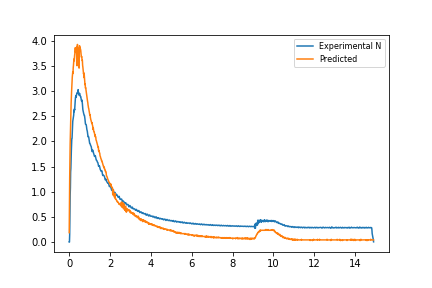
\includegraphics[scale=.5]{Figures/ExampleTemp}
\caption{Example plot of the temperature over time for a trial}
\label{fig:BadTemp}
\end{figure}
The limited resolution of the ADC can be seen quite clearly. However, this is not terribly problematic and several things can be done to smooth the curve. A function from the pandas python library that handles smoothing quite well was used to compensate for this. It uses a moving averages method. The smoothed plot is shown in figure \ref{fig:SmoothedTemp}.
\begin{figure}[h!]
\centering
\includegraphics[scale=.5]{Figures/SmoothTemp}
\caption{Example plot now smoothed}
\label{fig:SmoothedTemp}
\end{figure}
There are additional problems that come with smoothing data, though. The total number of points is typically reduced and therefore all of the data that is going to be used must then be smoothed by the same factor. Also, the data is shifted to the left as can be seen from figures \ref{fig:BadTemp} and \ref{fig:SmoothedTemp}. Alternatively, a function could be fit to the data and this would allow the possibility of a continuous data set. For now though, there are bigger problems with the data recorded. Figure \ref{fig:BothTemps} shows the two different temperature data sets plotted against time for one of the trials. 
\begin{figure}[h!]
\centering
\includegraphics[scale=.5]{Figures/TwoSmoothedTemps}
\caption{Smoothed $T_c$ and $T_e$ plotted with time for one of the trials}
\label{fig:BothTemps}
\end{figure}
It can be seen immediately that at some point the $T_c$ line drops below the $T_e$ line. Looking back at equation \ref{eq:NozzleForce} this is troublesome. This means that $\left(1-\frac{T_e}{T_c}\right)<0$ giving an overall negative sign under the square root. Obviously the force produced is not imaginary, so either the data collected for these temperatures is not representative of the actual variables or the theory is wrong. It is obvious that the former is the problem for several reasons. The first is that the $T_c$ variable represents the temperature directly before the converging section of the nozzle. $T_e$ is the temperature of the exit plane of the nozzle. The two thermocouples are not placed in these regions. Admittadely, there was not enough attention when inspecting the theory to develop the experiment. Under normal circumstances some simple changes would be made and new data would be taken, however due to the closure of the university nothing can be done about collecting new data. Because of this we will proceed with what analysis can be completed and use a more general approach to characterizing the CGT. First, I've plotted the predicted force with the experimental force in figure \ref{fig:FirstThrust}. 
\begin{figure}[h!]
\centering
\includegraphics[scale=.5]{Figures/FirstAttempt}
\caption{First attempt at plotting the thrust and predicted thrust against time}
\label{fig:FirstThrust}
\end{figure}
As expected, we see segments where the force is undefined due to a runtime error in the numpy package.
\subsection{Attempt at Reconciliation}
The most obvious way to resolve the negative sign is to include an absolute value around the problematic term. This solves the runtime error, but is unfounded. The optimum nozzle expansion ratio should have the largest thrust production, but  $T_e's$ dependence on the exit area is essentially removed on the expansion ratio in doing this. This means the thrust will be highest for the value which has the greatest expansion ratio which is geometry O4. This can be seen in figure \ref{fig:FirstThreeCurves}. Several trials have been plotted there and included the predicted force according to equation \ref{eq:NozzleForce}.
\begin{figure}[h!]
\centering
\includegraphics[scale=.5]{Figures/FirstThreeCurves}
\caption{Several trials thrust curves plotted with the predicted thrust}
\label{fig:FirstThreeCurves}
\end{figure}
O4 is indeed the largest thrust curve. Also, in viewing these thrust curves it is important to recognize the predicted force is the predicted force per unit mass, but the actual curve is per some different mass value. However, the unit for the mass can be set to some convenient unit and be compared through all the data. This won't change the actual analysis and design conditions.\\
Tacking on an absolute value will not only fail to resolve the issue here but it is also unfounded. The next thought is to solve for $T_e$ in terms of the other available variables. It turns out that $T_e$ can be put in terms of $T_c,\ P_c,\ A_e,\ \rho_c,\ and\ w$.%
\nomenclature{$w$}{Mass flow rate}
Unfortunately, there are several problems with this. The first is that the change in mass, the mass flow rate, was only measured as an initial and final value. Meaning the total mass used throughout the experiment is known, but the mass flow rate throughout is not. For now, the assumption will be made that the mass flow rate is constant. Next, as can be seen from equation \ref{eq:ExitTemp} $T_e$ cannot be solved algebraically. It is not difficult to solve for it computationally though. 
\begin{equation}\label{eq:ExitTemp}
T_e = T_c\left[\frac{\gamma -1}{2\gamma P_c \rho_c} \left(\frac{w}{A_e}\right)^2\left(\frac{T_c}{T_e}\right)^{\frac{\gamma+1}{\gamma-1}}+1\right]^{-1}
\end{equation}
The simplist method is to use the relaxation method as described in \cite{newman}. The process is to iterate the equation by plugging in $T_e=1$ on the right side, finding a new value for $T_e$ on the left side, substitutting this value back into the right side, and so on. $T_e$ should converge to a value and that is the solution for $T_e$. Using this method, I've made the same plots in figure \ref{fig:SecondThreeCurves} as in figure \ref{fig:FirstThreeCurves}.
\begin{figure}[h!]
\centering
\includegraphics[scale=.5]{Figures/SecondThreeCurves}
\caption{Several trials thrust curves plotted with the predicted thrust}
\label{fig:SecondThreeCurves}
\end{figure}
The similarity between the two figures is quite apparent. At first glance, they nearly look the same, but looking at the far right plot the theoretical curve can be seen to be different from the other. The reason for this is because the assumption made about the mass flow rate being constant through time was naive. The mass flow rate, at any point $x$  can be defined by equation \ref{eq:MassFlow}.
\begin{equation}\label{eq:MassFlow}
w_x=A_x v_x \rho_x
\end{equation}%
\nomenclature{$v$}{Gas velocity}%
\nomenclature{$X_x$}{Any variable, X at some point, x}
Both the velocity and density of the gas have dependence on pressure and temperature so $w$ is \textit{not} constant with respect to time. That is not to say it is not constant at any given time throughout the entire system, however. If $T_e$ is not represented correctly it is clear that the result is that the nozzle with the largest expansion ratio is predicted to function best because of equation \ref{eq:NozzleForce}'s dependence on $A_e$. \\
Unfortunately, this doesn't tell much because the theoretical values cannot be calculated for the same reasons as the force. Additionally, it is not ideal to look at the specific impulse over the entire experiment because the temperature and pressure are so transient. However, since the change in mass is only known for two data points it is the best that can be done. Determining these values is a simple trapezoidal sum over all time. I've tabulated all of these in table \ref{table:Isps}.
\begin{table}[!h]
\centering
\begin{tabular}{
>{\columncolor[HTML]{C0C0C0}}c 
>{\columncolor[HTML]{EFEFEF}}c 
>{\columncolor[HTML]{EFEFEF}}c }
Geometry & \cellcolor[HTML]{C0C0C0}$Trial\ 1\ I_{sp}$ & \cellcolor[HTML]{C0C0C0}$Trial\ 2\ I_{sp}$ \\
N        & 61.1                                       & 54.0                                       \\
U4       & 58.0                                       & 44.1                                       \\
U3       & 33.5                                       & 52.8                                       \\
U2       & 62.5                                       & 60.3                                       \\
U1       & 33.9                                       & 62.6                                       \\
O        & 57.5                                       & 37.3                                       \\
O1       & 58.6                                       & 59.5                                       \\
O2       & 50.5                                       & 48.3                                       \\
O3       & 29.0                                       & 60.3                                       \\
O4       & 44.6                                       & 56.0                                      
\end{tabular}
\caption{Experimental specific impulses}
\label{table:Isps}
\end{table}
In the end, there is not much reconciliation that can be done for the poor data collection.\\
There isn't much to see here, except that the values found are close to the known values from reference \cite{anis}. The $I_{sp}'s$ dependence on temperature and pressure means that these values are meaningless without the theoretical values at the same pressure and temperature. Reference \cite{anis} is using values for the maximum possible $I_{sp}$ values.

\chapter{Discussion}\label{chap:Discussion}
Unfortunately, due to COVID-19 the necessary corrections could not be made to the project. This means the system could not be characterized with the intended scheme. It can be seen, though, that the values found are close to the known values from reference \cite{anis}. The theoretical value provided there is $67\ s$ and the measured value is $61\ s$. Included in Table \ref{table:Isps} is a \% difference between the literature's theoretical value (\%Diff. T) and the average value determine for each geometry as well as a \% difference for the literature's experimental value and average value found (\%Diff M). \% differences as low as 1\% and as high as 36\% can be seen there. There are two reasons the results cannot be clearly compared. The first is the $I_{sp}'s$ dependence on temperature and pressure. Meaning that these values are meaningless without the theoretical values at the same pressure and temperature. Reference \cite{anis} is using values for the maximum possible $I_{sp}$ values. The second reason is that there was no error analysis performed here.\\
However, the importance of this research is the development of the system and  scripting. The focus on both readability and generalizability is the value here. Additionally, the work done here has allowed the realization of certain errors. The solutions to these errors are presented below.\\
The most obvious problems with this setup are shown in the analysis. The exit plane temperature is not well represented and neither is the mass flow rate. Additionally, the stagnation conditions for the actual system are not well-defined.
\section{Hardware}
Here, the problems regarding the hardware of the project are discussed.
\subsection{ADC}
The analog to digital converter is used to convert the analog voltage signals from the variable sensors to digital signals that the Raspberry Pi can read in. The resolution of the device is defined by the number of \textit{bits} it has. The MCP3008 is a 10-bit ADC used for the temperature sensors. Since it is a 10-bit ADC, the number of levels ($N$) available for storing voltage signals is 1024. In other words,
\begin{equation}
N=2^{bits}
\end{equation}
The HX711 is a 24-bit ADC, meaning $N=16777216$. The HX711 has the capability of being 16384x more accurate than the MCP3008. The poor resolution is clearly seen in the raw temperature plots, such as the one shown in Figure \ref{fig:BadTemp}. The reason the HX711 was not used for the temperature data, however was the open source library interfacing with it was meant to be used specifically for the load cell. The chip was also on a breakout board and did not have other channel options. Most of the 24-bit ADCs require the use of a standard communication protocol, I2C. Finding open source libraries for these higher resolution devices is difficult and the user would likely have to build one themselves. However, this is not completely out of reach as there are many sources providing information on the subject and implementations in Python do exist. This was not a complete necessity though and was put aside for future design iterations.
\subsection{Pressure Regulator}
The stagnation conditions discussed in Chapter \ref{chap:Theory}, were not well defined prior to the first run of trials. Because of this, data that is meant to be stagnant is not. Also, since the $CO_2$ was spent so quickly it caused some of it to fuse into a solid. This is definitely not ideal for several reasons. The first is that solid $CO_2$ can block plumbing and cause issues for the RCS. Next, is the previously mentioned issue of stagnation. If the $CO_2$ changes temperature so rapidly, the chamber pressure will also be decreasing rapidly. This creates an ill-defined stagnation condition and an optimum nozzle geometry is impossible to correctly determine. With the use of a pressure regulator the stagnation conditions could be clearly determined. Also, this could allow the use of a feedback system that would add heat to the system such as to condition the temperature to stay constant even through a continuous discharge. It may also be possible to create the same effect by decreasing the nozzle throat radius. Either way, this should most likely be done because the mass flow rate for the system is too high.
\section{Software}
Changes to the software include a better method for stopping each experiment. The current method as discussed in Chapter \ref{chap:Analysis} is to determine when the force value dropped below a certain threshold for a specified amount of time. The force sensor sometimes lost its zero position and created problems for stopping data collection. A more robust method would be using time derivatives of the force to classify when the data collection should end. This would create more consistent data files and plots. The scripts should also be updated for the addition of the new hardware mentioned above. Most importantly, is to begin an error analysis section. This would consist of new hardware scripts to determine the reliability of sensors and scripts performing error analysis on the actual functions used. This would not only allow the comparison between other literature values and the determined ones, but it would also allow the system a higher level of reliability. For example, determining how much fuel should be taken for mission objectives could be determined with higher confidence.

\chapter{Conclusion}\label{chap:Conclusion}
The over arching goal of this research project is to develop a reaction control system for high altitude balloons. The work completed includes an analysis on viability of the system, an experimental design, data collection, and analysis on it. The experimental design had errors associated with it and because of this the analysis did not provide system characterization. Next steps include correcting the experimental errors, finishing the analysis, integrating the CGT into a HABP, and flying the system. Additional thoughts on future work are the possibility of attempting another axis of stabilization. In this project, only two thrusters were ever really considered. This is because the payload does not see many perturbations in the upward or downward directions due to the nature of the balloon system. The biggest consideration here is not just fuel limitations but also the weight limitations. The heaviest part of the system is by far the solenoid; to add another axis of stabilization means adding two more solenoids. \\
In correcting the experimental errors, the options are not left open. There are clear solutions that can be proceeded with quickly. After this though, the project is much more open-ended. Actually integrating the cold gas thruster system into the high altitude balloon payload is not clearly defined here. There are several interesting methods to go about implementing this as an effective reaction control system and the carry-over is quite similar to the systems used to stabilize rockets, satellites, etc. Because of this there is paramount information available for proceeding. The many applications of the RCS show its robust nature and the possibilities with it.

\nocite{*}
\bibliographystyle{plain}
\bibliography{References}

\appendix
\chapter{Appendix Title}\label{chap:Appendix}
\section{Scripting}\label{sec:Scripting}
Here, two primary files are included. The first is the file that runs the experiment for data collection and the second is the analysis class for data analysis. The file, experiment.py, is shown below and is hosted at this \href{https://github.com/maxmhuggins/RCS_HAB/blob/master/On_Ground_Testing/Code/experiment.py}{URL}\footnote{Physical URL: \url{https://github.com/maxmhuggins/RCS_HAB/blob/master/On_Ground_Testing/Code/experiment.py}}.
\lstinputlisting[language=Python]{Scripts/experiment.py}
The next file, Analysis\_Class.py, is hosted at this \href{https://github.com/maxmhuggins/RCS_HAB/blob/master/On_Ground_Testing/Data_and_Analysis/Experimental_Data_Analysis/Scripts/Analysis_Class.py}{URL.}\footnote{Physical URL: \url{https://github.com/maxmhuggins/RCS_HAB/blob/master/On_Ground_Testing/Data_and_Analysis/Experimental_Data_Analysis/Scripts/Analysis_Class.py}} This file takes in all of the data recorded from experiment.py and is also shown below:
\lstinputlisting[language=Python]{Scripts/Analysis_Class.py}
\section{Schematics}\label{sec:Schematics}
Here, the most relevant circuit schematics are provided. Shown below is the entire circuit schematic used for interfacing the Raspberry Pi with the sensors, the power supply handling, and the push pull amplifier for the solenoid respectively.
\begin{figure}[!ht]
\centering
\includegraphics[width=6.5in]{Figures/DataCollection}
\caption{Circuit diagram including the MCP3008 ADC, HX711 breakout board, AD8495 breakout boards, TXS0108E 8 Channel Logic Level Converter, and a representation fo the pressure transducer. Pin 13 of the level shifter goes to the solenoid amplifier circuit in Figure \ref{fig:SolenoidSchem}}
\label{fig:DataCollectionSchem}
\end{figure}\clearpage
\begin{figure}[h!]
\centering
\includegraphics[width=6.5in]{Figures/PowerSupply}
\caption{LM317 linear voltage regulators being used for 3 separate supply voltages, 12V, 5V, and 3.3V.}
\label{fig:PowerSupplySchem}
\end{figure}
\begin{figure}[!ht]
\centering
\includegraphics[width=3.1in]{Figures/Solenoid}
\caption{Solenoid amplifier circuit used for ensuring the solenoid switches on/off completely and the digital logic pin from the RPi is not damaged in an attempt to source too much current.}
\label{fig:SolenoidSchem}
\end{figure}
\section{Parts List}\label{sec:PartsList}
Here a parts list is included of the purchased equipment for the project. Parts not shown here were available in the research lab at the university.
\begin{table}[!h]
\centering
\resizebox{\textwidth}{!}{%
\begin{tabular}{cclccc}
\rowcolor[HTML]{C0C0C0} 
Seller        & \multicolumn{1}{c}{\cellcolor[HTML]{C0C0C0}Item} & \multicolumn{1}{c}{\cellcolor[HTML]{C0C0C0}Description} & Price per Unit (USD) & Quantity                          & Subtotals (USD)                  \\
\rowcolor[HTML]{EFEFEF} 
McMaster-Carr & 7833K73                                          & High‐Pressure Precision Flow‐Adjustment Valve           & 28.73               & 2                                 & 57.46                           \\
\rowcolor[HTML]{EFEFEF} 
McMaster-Carr & 5220K158                                         & Inline Tee for 1/4" Copper Tube OD x 1/8 NPTF Male      & 10.00               & 1                                 & 10.00                           \\
\rowcolor[HTML]{EFEFEF} 
McMaster-Carr & 8955K112                                         & General Purpose Copper Tubing                           & 28.29               & 1                                 & 57.72                           \\
\rowcolor[HTML]{EFEFEF} 
McMaster-Carr & 5272K299                                         & Straight Adapter for 1/4" Tube OD x 1/8 NPT Male        & 4.81                & 12                                & 28.29                           \\
\rowcolor[HTML]{EFEFEF} 
McMaster-Carr & 5485K21                                          & Straight Connector, 1/8 NPT Male                        & 1.40                & 1                                 & 1.40                            \\
\rowcolor[HTML]{EFEFEF} 
McMaster-Carr & 50785K26                                         & Reducing Adapter, 1/4 NPT Female x 1/8 NPT Male         & 1.58                & 1                                 & 1.58                            \\
\rowcolor[HTML]{EFEFEF} 
McMaster-Carr & 50785K75                                         & Tee Connector, 1/8 NPT Female                           & 3.73                & 1                                 & 3.73                            \\
\rowcolor[HTML]{EFEFEF} 
McMaster-Carr & 1190N21                                          & Stainless Steel, 24V DC, 1/8 NPT Female, 3000 Max PSI   & 138.97              & 3                                 & 416.91                          \\
\rowcolor[HTML]{EFEFEF} 
Amazon        & B07K2JQ6CG                                       & 30 Packs x 16g Threaded CO2 Cartridges                  & 25.90               & 1                                 & 25.90                           \\
\rowcolor[HTML]{EFEFEF} 
Amazon        & B07PFY54TV                                       & 25g Threaded CO2 Cartridges, 6 Pack                     & 24.99               & 1                                 & 24.99                           \\
\rowcolor[HTML]{EFEFEF} 
Amazon        & B07DN3L9N2                                       & G 1/4" Male Thread x 1/4" NPT Female                    & 14.99               & 1                                 & 14.99                           \\
\rowcolor[HTML]{EFEFEF} 
Amazon        & B07GJGTWQT                                       & G1/4" Pressure Transducer Sensor (0‐1000psi)            & 23.19               & 1                                 & 23.19                           \\
\rowcolor[HTML]{EFEFEF} 
Amazon        & B07YGN2QGL                                       & UV Resin Curing Light for SLA/DLP 3D Printer            & 25.99               & 1                                 & 25.99                           \\
\rowcolor[HTML]{EFEFEF} 
Amazon        & B07KSYRW34                                       & Strong and Precise High Resolution 3D Printing Resin    & 49.95               & 2                                 & 49.95                           \\
\rowcolor[HTML]{EFEFEF} 
Amazon        & B06XWVZHZJ                                       & 8 Channel Logic Level Converter Bi‐Directional High     & 7.99                & 1                                 & 7.99                            \\
\rowcolor[HTML]{EFEFEF} 
Amazon        & B07K2ZHMRF                                       & ELEGOO Mars UV Photocuring LCD 3D Printer               & 229.99              & 1                                 & 229.99                          \\
              & \multicolumn{1}{c}{}                             & \multicolumn{1}{c}{}                                    &                     & \cellcolor[HTML]{C0C0C0}Subtotal: & \cellcolor[HTML]{C0C0C0}1030.03
\end{tabular}%
}
\caption{Some components purchased for use in this project, everything purchased from either McMaster-Carr or Amazon.}
\label{tab:PartsList}
\end{table}

\end{document}

